\documentclass{beamer}
%
% Choose how your presentation looks.
%
% For more themes, color themes and font themes, see:
% http://deic.uab.es/~iblanes/beamer_gallery/index_by_theme.html
%
\mode<presentation>
{
  \usetheme{Madrid}      % or try Darmstadt, Madrid, Warsaw, ...
  \usecolortheme{seahorse} % or try albatross, beaver, crane, ...
  \usefonttheme{serif}  % or try serif, structurebold, ...
  \setbeamertemplate{navigation symbols}{}
  \setbeamertemplate{caption}[numbered]
} 

\usepackage[english]{babel}
\usepackage{kotex}
\usepackage{tikz}
\usepackage{listings}
\usepackage{pgffor}
\usepackage{listings}
\usepackage{amsfonts}
\usepackage[linesnumbered,ruled,vlined]{algorithm2e}
\usepackage{algorithmic}



\lstset{ %
  backgroundcolor=\color{white},   % choose the background color; you must add \usepackage{color} or \usepackage{xcolor}
  basicstyle=\tiny,        % the size of the fonts that are used for the code
  breakatwhitespace=false,         % sets if automatic breaks should only happen at whitespace
  breaklines=true,                 % sets automatic line breaking
  captionpos=b,                    % sets the caption-position to bottom
  commentstyle=\color{gray},    % comment style
  deletekeywords={...},            % if you want to delete keywords from the given language
  escapeinside={\%*}{*)},          % if you want to add LaTeX within your code
  extendedchars=true,              % lets you use non-ASCII characters; for 8-bits encodings only, does not work with UTF-8
  frame=single,                    % adds a frame around the code
  keepspaces=true,                 % keeps spaces in text, useful for keeping indentation of code (possibly needs columns=flexible)
  keywordstyle=\color{blue},       % keyword style
  language=C++,                 % the language of the code
  morekeywords={*,...},            % if you want to add more keywords to the set
  numbers=left,                    % where to put the line-numbers; possible values are (none, left, right)
  numbersep=5pt,                   % how far the linxe-numbers are from the code
  numberstyle=\tiny\color{gray}, % the style that is used for the line-numbers
  rulecolor=\color{black},         % if not set, the frame-color may be changed on line-breaks within not-black text (e.g. comments (green here))
  showspaces=false,                % show spaces everywhere adding particular underscores; it overrides 'showstringspaces'
  showstringspaces=false,          % underline spaces within strings only
  showtabs=false,                  % show tabs within strings adding particular underscores
  stepnumber=0,                    % the step between two line-numbers. If it's 1, each line will be numbered
  stringstyle=\color{gray},     % string literal style
  tabsize=2,                       % sets default tabsize to 2 spaces
  }

\title[3D 그래픽스 프로그래밍]{그래픽스 강의노트 10 - 프래그먼트 조작}
\author{강영민}
\institute{동명대학교}
\date{2015년 2학기}

\begin{document}

%%%%%%%%%%%%%%%%%%%%%%%%%%%%%%%%%%%%%%%%%%%%%%%%%%%%%%%%%
\begin{frame}
  \titlepage
\end{frame}

% Uncomment these lines for an automatically generated outline.
%\begin{frame}{Outline}
%  \tableofcontents
%\end{frame}





%%%%%%%%%%%%%%%%%%%%%%%%%%%%%%%%%%%%%%%%%%%%%%%%%%%%%%%%%
\begin{frame}[fragile]{프래그먼트}

\begin{itemize}
\item 화면 화소의 색은 프레임 버퍼에 기록되는 순간 결정
\item 프레임 버퍼에 기록되기 이전 단계의 추상적 개념의 화소: 프래그먼트
\item 화소의 위치, 색, 깊이, 텍스처 등 픽셀을 결정하기 위해 필요한 모든 정보를 가진 기본 단위
\end{itemize}


\end{frame}
%%%%%%%%%%%%%%%%%%%%%%%%%%%%%%%%%%%%%%%%%%%%%%%%%%%%%%%%%

%%%%%%%%%%%%%%%%%%%%%%%%%%%%%%%%%%%%%%%%%%%%%%%%%%%%%%%%%
\begin{frame}[fragile]{오픈지엘 버퍼}

\begin{itemize}
\item 스텐실버퍼
\item 
\end{itemize}

\end{frame}
%%%%%%%%%%%%%%%%%%%%%%%%%%%%%%%%%%%%%%%%%%%%%%%%%%%%%%%%%



%%%%%%%%%%%%%%%%%%%%%%%%%%%%%%%%%%%%%%%%%%%%%%%%%%%%%%%%%
\begin{frame}[fragile]{텍스처 유니트별로 텍스처 설정}

\lstset{language=C++, escapechar=^} 
\begin{lstlisting}
\// filename: main.cpp

void init(int argc, char **argv) {
  initWindow(&argc, argv);
  ...
  // ^{\it 텍스처 유니트 0에 텍스처를 하나 할당}^
  glActiveTexture(GL_TEXTURE0);
  tex1 = setTexture("surface.jpg");

  // ^{\it 텍스처 유니트 1에 텍스처를 하나 할당}^
  glActiveTexture(GL_TEXTURE1);
  tex2 = setTexture("spheremap.jpg");

  LightSet();
  glEnable(GL_DEPTH_TEST);
}
\end{lstlisting}

\end{frame}
%%%%%%%%%%%%%%%%%%%%%%%%%%%%%%%%%%%%%%%%%%%%%%%%%%%%%%%%%

%%%%%%%%%%%%%%%%%%%%%%%%%%%%%%%%%%%%%%%%%%%%%%%%%%%%%%%%%
\begin{frame}[fragile]{텍스처 유니트별로 텍스처 좌표 설정}

\lstset{language=C++, escapechar=^} 
\begin{lstlisting}
    glEnable(GL_TEXTURE_2D);
    glActiveTexture(GL_TEXTURE0);
    glBindTexture(GL_TEXTURE_2D, tex1);
    glActiveTexture(GL_TEXTURE1);
    glBindTexture(GL_TEXTURE_2D, tex2);
    glEnable(GL_TEXTURE_GEN_S);  glEnable(GL_TEXTURE_GEN_T);
    glTexGenf(GL_S, GL_TEXTURE_GEN_MODE,  GL_SPHERE_MAP);
    glTexGenf(GL_T, GL_TEXTURE_GEN_MODE,  GL_SPHERE_MAP);
    glutSolidTeapot(1.2);
    glDisable(GL_TEXTURE_GEN_S);  glDisable(GL_TEXTURE_GEN_T);
\end{lstlisting}

\end{frame}
%%%%%%%%%%%%%%%%%%%%%%%%%%%%%%%%%%%%%%%%%%%%%%%%%%%%%%%%%

%%%%%%%%%%%%%%%%%%%%%%%%%%%%%%%%%%%%%%%%%%%%%%%%%%%%%%%%%
\begin{frame}[fragile]{텍스처 유니트별로 텍스처 좌표 설정 결과}

\begin{figure}[h!]
  \centering
	\begin{tabular}{cc}
	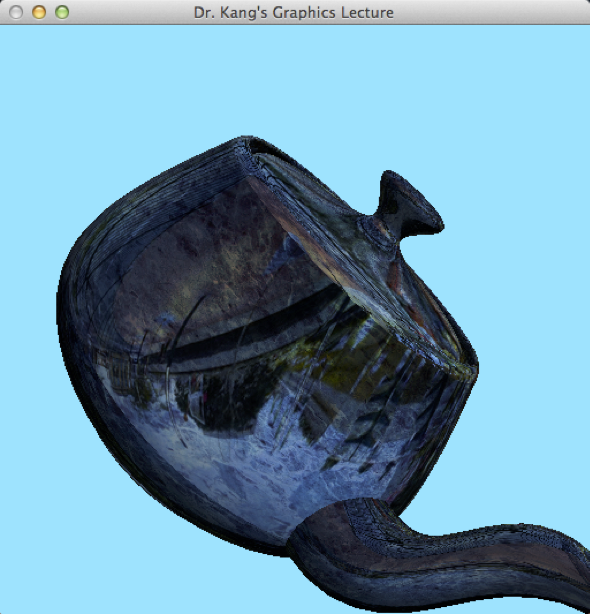
\includegraphics[height=6cm]{OGL_texture/multiTexturedA.png} &
	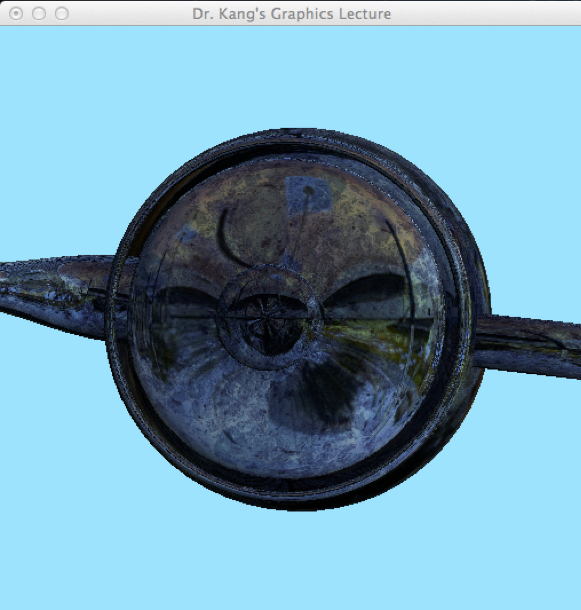
\includegraphics[height=6cm]{OGL_texture/multiTexturedB.png}  \\
	\end{tabular}
\end{figure}

\end{frame}
%%%%%%%%%%%%%%%%%%%%%%%%%%%%%%%%%%%%%%%%%%%%%%%%%%%%%%%%%

%%%%%%%%%%%%%%%%%%%%%%%%%%%%%%%%%%%%%%%%%%%%%%%%%%%%%%%%%
\begin{frame}[fragile]{텍스처 좌표를 명시적으로 달리 설정하는 법}

사용될 텍스처
\begin{figure}[h!]
  \centering
	\begin{tabular}{cc}
	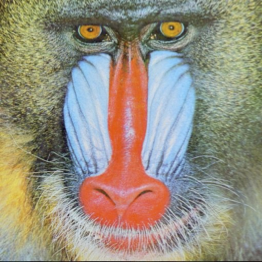
\includegraphics[height=5cm]{OGL_texture/multiTex2A.png} &
	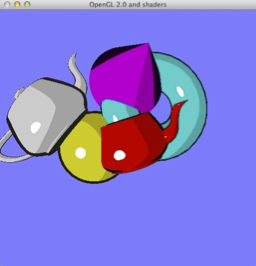
\includegraphics[height=5cm]{OGL_texture/multiTex2B.png}  \\
	\end{tabular}
\end{figure}

\end{frame}
%%%%%%%%%%%%%%%%%%%%%%%%%%%%%%%%%%%%%%%%%%%%%%%%%%%%%%%%%


%%%%%%%%%%%%%%%%%%%%%%%%%%%%%%%%%%%%%%%%%%%%%%%%%%%%%%%%%
\begin{frame}[fragile]{텍스처 좌표를 명시적으로 달리 설정하는 법}

\lstset{language=C++} 
\begin{lstlisting}
	glBegin(GL_QUADS);
	glNormal3f(0.0, 0.0, 1.0);
	glMultiTexCoord2f(GL_TEXTURE0, 0.0, 0.0);
	glMultiTexCoord2f(GL_TEXTURE1, 0.0, 0.0);
	glVertex3f(-0.5, 0.5, 0.0);
	glMultiTexCoord2f(GL_TEXTURE0, 0.0, 1.0);
	glMultiTexCoord2f(GL_TEXTURE1, 0.0, 2.0);
	glVertex3f(-0.5,-0.5, 0.0);
	glMultiTexCoord2f(GL_TEXTURE0, 1.0, 1.0);
	glMultiTexCoord2f(GL_TEXTURE1, 2.0, 2.0);
	glVertex3f( 0.5,-0.5, 0.0);
	glMultiTexCoord2f(GL_TEXTURE0, 1.0, 0.0);
	glMultiTexCoord2f(GL_TEXTURE1, 2.0, 0.0);
	glVertex3f( 0.5, 0.5, 0.0);
	glEnd();
\end{lstlisting}

\end{frame}
%%%%%%%%%%%%%%%%%%%%%%%%%%%%%%%%%%%%%%%%%%%%%%%%%%%%%%%%%

%%%%%%%%%%%%%%%%%%%%%%%%%%%%%%%%%%%%%%%%%%%%%%%%%%%%%%%%%
\begin{frame}[fragile]{텍스처 좌표를 명시적으로 달리 설정하는 법}

\begin{figure}[h!]
  \centering
	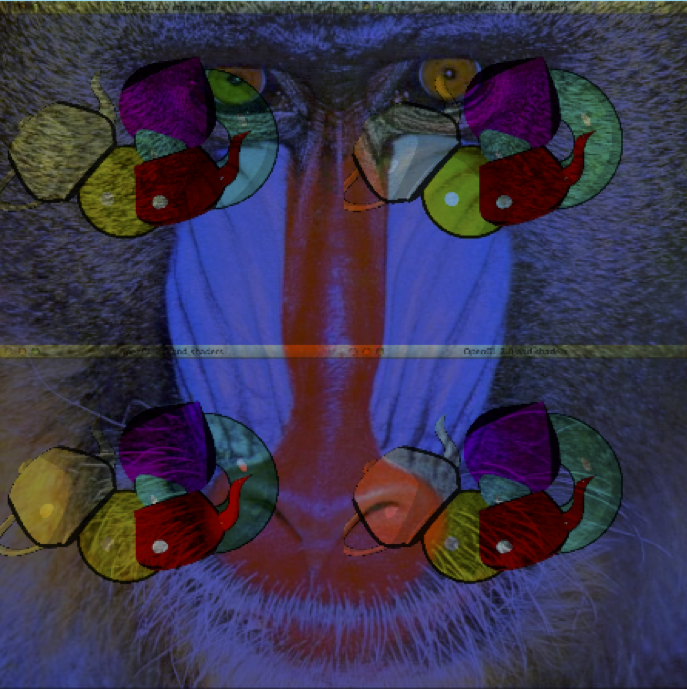
\includegraphics[height=6cm]{OGL_texture/multiTex2.png} 
\end{figure}

\end{frame}
%%%%%%%%%%%%%%%%%%%%%%%%%%%%%%%%%%%%%%%%%%%%%%%%%%%%%%%%%


%%%%%%%%%%%%%%%%%%%%%%%%%%%%%%%%%%%%%%%%%%%%%%%%%%%%%%%%%
\begin{frame}[fragile]{텍스처 좌표의 변환}

\lstset{language=C++} 
\begin{lstlisting}
glBegin(GL_QUADS);
glMultiTexCoord2f(GL_TEXTURE0, 0.0, 0.0);
glMultiTexCoord2f(GL_TEXTURE1, 0.0, 0.0);
glVertex3f(-0.5, 0.5, 0.0);
glMultiTexCoord2f(GL_TEXTURE0, 0.0, 1.0);
glMultiTexCoord2f(GL_TEXTURE1, 0.0, 1.0);
glVertex3f(-0.5,-0.5, 0.0);
glMultiTexCoord2f(GL_TEXTURE0, 1.0, 1.0);
glMultiTexCoord2f(GL_TEXTURE1, 1.0, 1.0);
glVertex3f( 0.5,-0.5, 0.0);
glMultiTexCoord2f(GL_TEXTURE0, 1.0, 0.0);
glMultiTexCoord2f(GL_TEXTURE1, 1.0, 0.0);
glVertex3f( 0.5, 0.5, 0.0);
glEnd();
\end{lstlisting}

\lstset{language=C++, escapechar=^} 
\begin{lstlisting}
    glActiveTexture(GL_TEXTURE0);
    glBindTexture(GL_TEXTURE_2D, tex1);
    glActiveTexture(GL_TEXTURE1);
    glBindTexture(GL_TEXTURE_2D, tex2);
    ^{\bf \color{red} glMatrixMode(GL\_TEXTURE)}^; //^{\it 행렬 모드를 텍스처 모드로 바꾼다}^
    glLoadIdentity();
    glScalef(5.0, 5.0, 1.0);    
    glBegin(GL_QUADS);
    ^{\sf 앞의 코드와 같은 내용으로 작성}^
    glEnd();
\end{lstlisting}

\end{frame}
%%%%%%%%%%%%%%%%%%%%%%%%%%%%%%%%%%%%%%%%%%%%%%%%%%%%%%%%%


%%%%%%%%%%%%%%%%%%%%%%%%%%%%%%%%%%%%%%%%%%%%%%%%%%%%%%%%%
\begin{frame}[fragile]{텍스처 좌표의 변환}

\begin{figure}[h!]
    \centering
	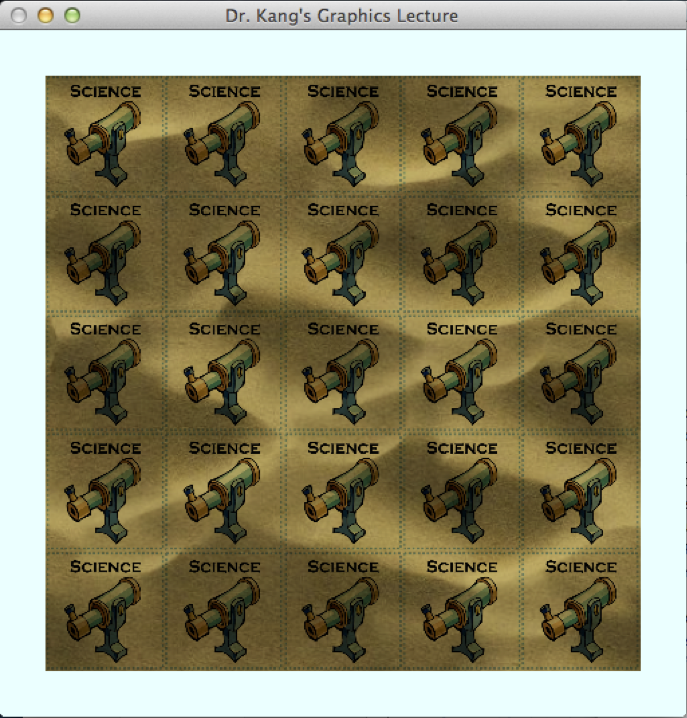
\includegraphics[height=6cm]{OGL_texture/multiTexturedForAni.png} 
\end{figure}

\end{frame}
%%%%%%%%%%%%%%%%%%%%%%%%%%%%%%%%%%%%%%%%%%%%%%%%%%%%%%%%%


%%%%%%%%%%%%%%%%%%%%%%%%%%%%%%%%%%%%%%%%%%%%%%%%%%%%%%%%%
\begin{frame}[fragile]{텍스처 애니메이션}

\lstset{language=C++} 
\begin{lstlisting}
glActiveTexture(GL_TEXTURE0);
glMatrixMode(GL_TEXTURE);
glLoadIdentity();
glScalef(1.0+sin(t)*0.1, 1.0+sin(t)*0.1, 1.0);
	
glActiveTexture(GL_TEXTURE1);
glMatrixMode(GL_TEXTURE);
glLoadIdentity();
glTranslatef(t,0,0);
glScalef(5.0, 5.0, 1.0);
glEnd();
\end{lstlisting}

\begin{figure}[h!]
    \centering
	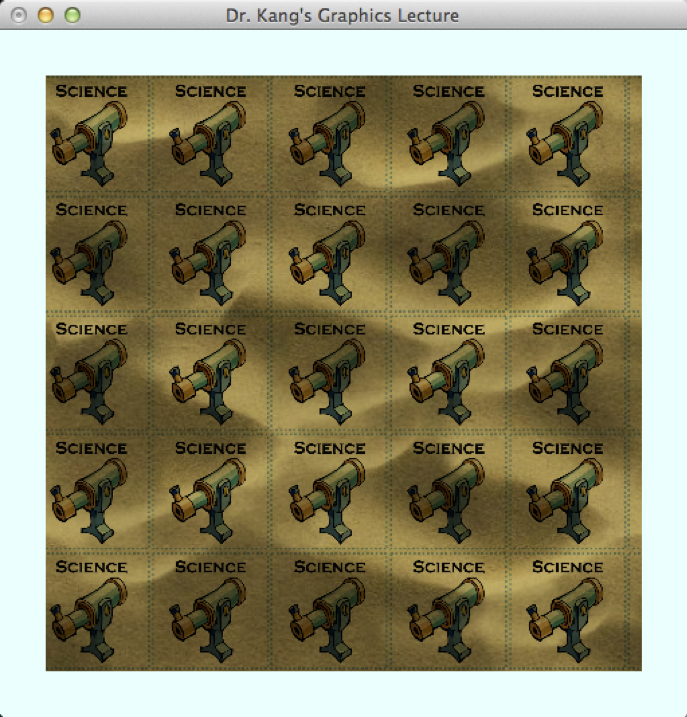
\includegraphics[height=4cm]{OGL_texture/multiTexAni_A.png} 
	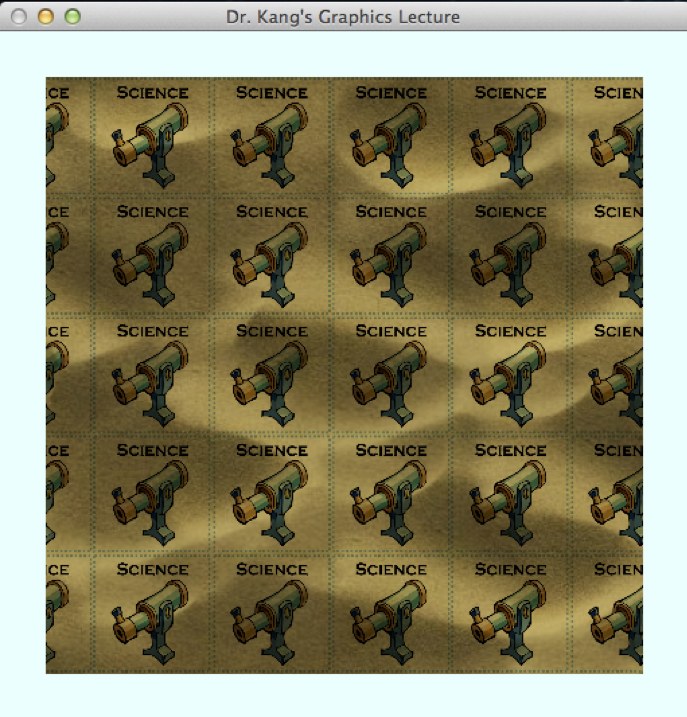
\includegraphics[height=4cm]{OGL_texture/multiTexAni_B.png} 
\end{figure}

\end{frame}
%%%%%%%%%%%%%%%%%%%%%%%%%%%%%%%%%%%%%%%%%%%%%%%%%%%%%%%%%
\end{document}



